\documentclass{article}\usepackage[]{graphicx}\usepackage[]{color}
% maxwidth is the original width if it is less than linewidth
% otherwise use linewidth (to make sure the graphics do not exceed the margin)
\makeatletter
\def\maxwidth{ %
  \ifdim\Gin@nat@width>\linewidth
    \linewidth
  \else
    \Gin@nat@width
  \fi
}
\makeatother

\definecolor{fgcolor}{rgb}{0.345, 0.345, 0.345}
\makeatletter
\@ifundefined{AddToHook}{}{\AddToHook{package/xcolor/after}{\definecolor{fgcolor}{rgb}{0.345, 0.345, 0.345}}}
\makeatother
\newcommand{\hlnum}[1]{\textcolor[rgb]{0.686,0.059,0.569}{#1}}%
\newcommand{\hlstr}[1]{\textcolor[rgb]{0.192,0.494,0.8}{#1}}%
\newcommand{\hlcom}[1]{\textcolor[rgb]{0.678,0.584,0.686}{\textit{#1}}}%
\newcommand{\hlopt}[1]{\textcolor[rgb]{0,0,0}{#1}}%
\newcommand{\hlstd}[1]{\textcolor[rgb]{0.345,0.345,0.345}{#1}}%
\newcommand{\hlkwa}[1]{\textcolor[rgb]{0.161,0.373,0.58}{\textbf{#1}}}%
\newcommand{\hlkwb}[1]{\textcolor[rgb]{0.69,0.353,0.396}{#1}}%
\newcommand{\hlkwc}[1]{\textcolor[rgb]{0.333,0.667,0.333}{#1}}%
\newcommand{\hlkwd}[1]{\textcolor[rgb]{0.737,0.353,0.396}{\textbf{#1}}}%
\let\hlipl\hlkwb

\usepackage{framed}
\makeatletter
\newenvironment{kframe}{%
 \def\at@end@of@kframe{}%
 \ifinner\ifhmode%
  \def\at@end@of@kframe{\end{minipage}}%
  \begin{minipage}{\columnwidth}%
 \fi\fi%
 \def\FrameCommand##1{\hskip\@totalleftmargin \hskip-\fboxsep
 \colorbox{shadecolor}{##1}\hskip-\fboxsep
     % There is no \\@totalrightmargin, so:
     \hskip-\linewidth \hskip-\@totalleftmargin \hskip\columnwidth}%
 \MakeFramed {\advance\hsize-\width
   \@totalleftmargin\z@ \linewidth\hsize
   \@setminipage}}%
 {\par\unskip\endMakeFramed%
 \at@end@of@kframe}
\makeatother

\definecolor{shadecolor}{rgb}{.97, .97, .97}
\definecolor{messagecolor}{rgb}{0, 0, 0}
\definecolor{warningcolor}{rgb}{1, 0, 1}
\definecolor{errorcolor}{rgb}{1, 0, 0}
\makeatletter
\@ifundefined{AddToHook}{}{\AddToHook{package/xcolor/after}{
\definecolor{shadecolor}{rgb}{.97, .97, .97}
\definecolor{messagecolor}{rgb}{0, 0, 0}
\definecolor{warningcolor}{rgb}{1, 0, 1}
\definecolor{errorcolor}{rgb}{1, 0, 0}
}}
\makeatother
\newenvironment{knitrout}{}{} % an empty environment to be redefined in TeX

\usepackage{alltt}


\usepackage{arxiv}
\usepackage[utf8]{inputenc} % allow utf-8 input
\usepackage[T1]{fontenc}    % use 8-bit T1 fonts
\usepackage{hyperref}       % hyperlinks
%\usepackage{url}            % simple URL typesetting
\usepackage{booktabs}       % professional-quality tables
\usepackage{amsfonts}       % blackboard math symbols
%\usepackage{nicefrac}       % compact symbols for 1/2, etc.
%\usepackage{microtype}      % microtypography



\usepackage{float}
\usepackage{framed}
\usepackage{subcaption}
\usepackage{amsmath, amsthm,amssymb}
\usepackage{parskip}
\usepackage{graphicx}
\usepackage{listings}
\usepackage{enumitem}
\usepackage{setspace}
\usepackage[english]{babel}

\DeclareMathOperator*{\argmax}{argmax}
\newcommand{\prog}[1]{\textsf{#1}}
\def\bigr{{\mathbb{R}}}
\newcommand{\pkg}[1]{\textbf{\emph{#1}}}
\newcommand{\class}[1]{`\code{#1}'}
\newcommand{\fct}[1]{\textit{#1()}}
\def\reml{{\text{reml}}}
\def\N{{\mathrm{N}}}
\def\MVN{{\mathrm{MVN}}}
\def\var{{\mathrm{Var}}}
\def\cov{{\mathrm{COV}}}
\def\Pr{{\mathbb{P}}}
\def\T{{\footnotesize {^{_{\sf T}}}}}
\def\E{\mathbb{E}} % expectation
\newcommand{\mathleft}{\@fleqntrue\@mathmargin0pt}



\newcommand\sectionprelude{%
  \vspace{1.5em}
}

\newtheorem{theorem}{Theorem}[section]
\newtheorem*{theorem*}{Theorem}



\title{A title}
\date{}

\author{
  Ruoyong Xu\\
  Department of Statistical Sciences\\
  University of Toronto\\
  700 University Ave., Toronto, ON M5G 1Z5, Canada\\
  \texttt{ruoyong.xu@mail.utoronto.ca} \\
  %% examples of more authors
   \And
  Patrick Brown\\
  Department of Statistical Sciences\\
  University of Toronto\\
  700 University Ave., Toronto, ON M5G 1Z5, Canada\\
  \texttt{patrick.brown@utoronto.ca} \\
}
\IfFileExists{upquote.sty}{\usepackage{upquote}}{}
\begin{document}
\maketitle
\setstretch{1.1}



\begin{abstract}
some keypoints to mention:\\
1, anisotropic spatial models are important but diffcult to evaluate because it consists of many covariance parameters.\\
2, standard approximations of spatial models (GMRF) don’t allow for anisotropy (at least as implemented). \\
3, gpuBatchMatrix is able to compute the profile LogL for each of the parameters in linear anisotropic spatial models, for dense matrix, use no approximation methods. allow for uncertainty in covariance parameters\\
4, investigated likelihood-based CI’s for variance parameters, wider than using information matrix based methods (gepstatsp)\\
\end{abstract}


% keywords can be removed
\keywords{First keyword \and Second keyword \and More}


\section{Introduction}
1- cI for the betas for the geostapsp package\\
2- Ci’s using profile likelihoods from gpuBatchMatrix
… second CI’s will be wider\\
… simulation study, profile CI’s have better coverage\\


emphasis for paper 2?
- anisotropic spatial models are important\\
- standard approximations of spatial models (GMRF) don’t allow for anisotropy (at least as implemented).  \\
- We do dense matrix, no approximations\\
- also, uncertainty in covariance parameters is important in anisotropic models because there are more of them.\\


- we should always allow for uncertainty in covariance parameters theta = sd, nugget, range, ratio, angle, shape, BoxCox\\
- … although most frequentist spatial software doesn’t, assumes theta = theta hat\\
- anisotropic models + boxcox + matern shape means many covariance parameters (7?)\\
- … important to understand uncertainty in covariance parameters, 2D profile L interesting\\
- … allow for uncertainty in covariance parameters to be reflected in CI’s for betas\\


- The easy way:  %L_easy(beta) = L(theta hat, beta), where theta hat = argmax_theta, beta L(theta, beta), numerically optimize over nu, range, shape,….., then plug in and estimate beta sigma again)\\
- Hard way:\\  %L_p(beta) =  L( theta(beta), beta)\\
Likelihood-based CI’s for variance parameters\\

We can estimate shape, range, variance\\
… likelihood might be fairly flat, CI’s are wide\\
… but CI’s have good coverage




\section{The linear geostatistical model}
\label{section1}
We start with a review of the linear geostatistical model:
%
\begin{gather*}
Y_{i}|U(s_i) \overset{ind}\sim \N(\lambda(s_{i}),\tau^2 ),\\
\lambda(s_{i})=X(s_i)\beta+U(s_{i}),\\
(U(s_1), \dots,U(s_n))^\T \sim \MVN (0,\Sigma),\\
\Sigma_{ij}=\cov \left[U(s_i), U(s_j)\right]=\begin{cases} 
\sigma^2 R(\|s_i-s_j\|/\phi;\kappa),& i\neq j .\\
\sigma^2, & i=j.
\end{cases}
\end{gather*}
%
where
$Y_i: i=1,\dots,n$ is the observation obtained at location $s_i$. 
Given $U(s_i)$, $Y_i$'s are mutually independently distributed with Gaussian distribution with observation variance $\tau^2$.  
$X(s_i)$ is a $1 \times p$ vector of explanatory variables at location $s_i$, 
$\beta=(\beta_1,\dots,\beta_p)^\T$ is the corresponding vector of regression parameters. 
$U=(U(s_1), \dots,U(s_n))^\T $ is a zero-mean Gaussian random field with covariance matrix $\Sigma$. The covariance between locations $(s_i)$ and $(s_j)$ takes the above form, where $R(\cdot)$ is the correlation function, and $\sigma^2$ is the spatial variance or variability in residual variation.  

Let $Y=(Y_1,\dots,Y_n)^\T$ be a vector of observations, and $X = (X(s_1), \dots, X(s_n))$ be an $n \times p$ design matrix, we rewrite the model in matrix format
%
\begin{equation*} 
Y \sim \MVN (X\beta, \sigma^2 R(\phi,\kappa)+\tau^2I).
\end{equation*}
% 
Write $V=R(\phi,\kappa)+\nu^2I$, and $\nu^2={\tau^2}/{\sigma^2}$, then
\begin{equation} \label{eq:1}
Y \sim \MVN (X\beta, \sigma^2 V).
\end{equation}





\subsection{Mat\'ern correlation}
The powered exponential family, the Mat\'ern family and the spherical family are the three most commonly used families of correlation functions in geostatistics. We favour the Mat\'ern family because of its flexibility, and it is made available in our \prog{R} package \pkg{gpuBatchMatrix}. The form of Mat\'ern correlation used in \pkg{gpuBatchMatrix} is 
\begin{equation*}
R(d;\phi,\kappa)=\frac{2^{\kappa-1}}{\Gamma(\kappa)} (\sqrt{8\kappa} \frac{d}{\phi})^\kappa  K_\kappa(\sqrt{8\kappa}  \frac{d}{\phi}),  \quad \text{where} \quad \phi>0,  \kappa > 0,
\end{equation*} 
$K_\kappa(\cdot)$ denotes the modified Bessel function of the second kind of order $\kappa$, 
$\kappa$ is the shape parameter which determines the smoothness of $U(x)$. For $\kappa=0.5$, the Mat\'ern correlation function coincides with the exponential correlation $\exp(-d/\phi)$. When $\kappa \rightarrow \infty$, it tends to the Gaussian correlation $\exp{\{-2(\|d\|/\phi)^2\}}$.
$\phi$ is called the range or scale parameter, it controls the rate of decay of the correlation as $d$ increases. 
%$d =\|x-x'\|$ is the Euclidean distance between two spatial points, $\Gamma(\cdot)$ is the standard gamma function,  $\phi$ is the range parameter or scale parameter with the dimension of distance, it controls the rate of decay of the correlation as $d$ increases. $K_\kappa(\cdot)$ is the modified Bessel function of the second kind with order $\kappa$, $\kappa$ is the shape parameter which determines the smoothness of $U(x)$, specifically, $U(x)$ is $m$ times mean-square differentiable if and only if $\kappa > m$.  Estimation of $\kappa$ is difficult, our experience is to choose the values of $\kappa$ from a discrete set, for example $\{0.5,1.5,2.5,\dots \}$(ref), %and then maximize the log-likelihood function \eqref{profile} or \eqref{remlpro} over $\phi$ and $\nu^2$. When the number of location points is large, the computation for the Mat\'ern function ...... more stuff ....


\subsection{Box-Cox transformation}
% What are the Box-Cox power transformations? The inference on the transformations parameter?
The fit of the linear geostatistical model can often be improved by applying a transformation to the response variable $Y$. Skewed random fields that mildly deviate from the Gaussian distribution can be modeled by means of the Box-Cox transformation (BCT) \cite{box1964analysis}.
%\cite{cressie2015statistics} introduced the term trans-Gaussian model to refer to the linear geostatistical model with a Box-Cox transformed  response variable. 
For positive-valued response variable $Y$, the Box-Cox transformation has the form
\begin{equation*}
    Y'=
    \begin{cases}
      (Y^\lambda-1)/\lambda: & \lambda \in \bigr \quad \text{and} \quad \lambda \neq  0, \\
      \log Y: & \lambda =0,
    \end{cases}
\end{equation*}
where $Y'$ denotes the transformed response. The aim of the BCT is to make data closely resemble the Gaussian distribution, so that the usual assumptions for linear models hold. The BCT cannot guarantee that any probability distribution can be normalized. However, even in cases when an exact mapping to the normal distribution is not possible, BCT may still provide a useful approximation \cite{hristopulos2020random}.


%The transformation parameter can be estimated by using maximum likelihood estimation. The log-likelihood including $\lambda$ is
% \begin{equation*}
% -2\ell^*(\beta,\sigma^2,V,\lambda)= -2*(\lambda-1)\sum_{i=1}^{n}\log y_i + n\log(2\pi)+\log |\sigma^2 V|+(y'-X\beta)^\T(\sigma^2 V)^{-1}(y'-X\beta),
% \end{equation*}




\subsection{Geometric anisotroy}
Geometrical anisotropy is defined by two additional parameters in the correlation function. Let $(x_1, x_2)$ represent the original coordinates, which is rotated counterclockwise by $\varphi$, then the new coordinates $(x'_1, x'_2)$ is given by
%
  \begin{equation*}\label{eq:matrixeqn}
    \begin{pmatrix}
      x'_{1} \\
      x'_{2}  
    \end{pmatrix}
    =
    \begin{pmatrix}
      1/\phi_{1} & 0 \\
      0 & 1/ \phi_{2} 
    \end{pmatrix}
    \cdot
    \begin{pmatrix}
      \cos \varphi & -\sin \varphi \\
      \sin \varphi & \cos \varphi 
    \end{pmatrix}
    \cdot
      \begin{pmatrix}
      x_1 \\
      x_2 
    \end{pmatrix},
  \end{equation*}
%
where $\varphi \in [-\pi/2, \pi/2]$ is called the anisotropy angle, $\psi = \phi_1 / \phi_2 \in [0,1]$ is the anisotropy ratio. %Anisotropy in correlation functions Statistical anisotropy can also be present in the correlation functions, where it is more difficult to estimate accurately. 

\section{Inference based on the likelihood function}
Let $y'^\T=(y'_1,\dots,y'_n)$ be the Box-Cox transformed data of the observations $y^\T=(y_1,\dots,y_n)$. The most general log-likelihood function for the linear geostatistical model parameters given $y'$ would be
%
\begin{equation}
-2\ell(\beta,\sigma^2, \lambda, \omega; y')=(y'-X\beta)^\T(\sigma^2 V)^{-1}(y'-X\beta)+\log |\sigma^2 V|-2*(\lambda-1)\sum_{i=1}^{n}\log y_i+n\log(2\pi).\label{eq:2}
\end{equation}
%
the third term on the right-hand side of \eqref{eq:2} arises from the Jacobian of the transformation. This log-likelihood function is complex to evaluate as we have several types of parameters to estimate, including the regression parameters $\beta$, the transformation parameter $\lambda$, and the covariance parameters $(\sigma^2, \phi,\kappa,\nu^2, \varphi, \psi)$. For simplicity we use $\omega=(\phi,\kappa,\nu^2, \varphi, \psi)$ to denote the correlation parameters in the following. 





\subsection{Profile log-likelihood functions}
%ADD gpuBatchMatrix and MORE STUFF\\
%"a gradient-based optimization algorithm can be used to reduce the computational cost of the optimization\\
%Another way to reduce the computational effort involved in the maximisation of l is to reduce the dimensionality of the optimization problem as follows."\\
The profile log-likelihood for parameter $\varphi$ is defined as $\ell_p(\varphi;y) = \underset{\psi}{\text{sup}} \ell (\varphi, \psi; y ).$ Given $\omega$ and $\lambda$, The log-likelihood function \eqref{eq:2} is maximized at
%
\begin{gather}
\hat{\beta}_{\omega,\lambda}=(X^\T V^{-1}X)^{-1} X^\T V^{-1}y', \quad \text{and} \label{betahat}\\
\hat{{\sigma}}^2_{\omega,\lambda}= \frac{1}{n}(y'-X\hat{\beta}_{\omega,\lambda})^\T V^{-1}(y'-X\hat{\beta}_{\omega,\lambda}) \label{eq:4}.
\end{gather}
%
%For simplicity, $\hat{\beta}_{w,\lambda}$ is written as $\hat{\beta}$ in \eqref{eq:4}, it denotes the maximum likelihood estimate of $\beta$ for a given $(w, \lambda)$. 
Substitute \eqref{betahat} and \eqref{eq:4} back into \eqref{eq:2}, we have the profile log-likelihood for $\omega$ and $\lambda$
%
\begin{equation} \label{profile}
-2\ell_p(\omega, \lambda;y')=n \log\frac{(y'-X\hat{\beta}_{\omega,\lambda})^\T V^{-1}(y'-X\hat{\beta}_{\omega,\lambda})}{n}+\log|V| -2(\lambda-1)\sum_{i=1}^{n}\log y_i + n\log(2\pi) + n,
\end{equation}
%

%\subsection{Restricted maximum likelihood estimation}
The main problem of maximum likelihood estimation is that variance is underestimated. Think of the simple case when the covariance matrix of $Y$ is $\sigma^2 I$, then 
\begin{align*}
&\hat{\sigma}^2 = \frac{1}{n}(y-X\hat{\beta})^\T (y-X\hat{\beta}),\\
&\E[\hat{\sigma}^2]=\frac{n-p}{n} \sigma^2 < \sigma^2,
\end{align*}
where $p= \text{rank}(X)$, is the number of elements in $\beta$. The estimation bias comes from not taking into account the degree of freedom used for estimating $\beta$. Restricted maximum likelihood (REML) developed by \cite{patterson1971recovery} is an approach that produces unbiased estimators or less biased estimators than MLE in general. REML eliminates the influence of $X$ on $\hat{\sigma}^2$ and $\hat{\omega}$. In this method, we find a matrix $A$ of full rank such that $AX=0$. The $n \times n$ projection matrix $S= I-X(X^\T X)^{-1}X^\T$ satisfies $SX=0$, however, $S$ is degenerate as $\text{rank}(S)=n-p$, so we take just $n-p$ linearly independent rows from $S$ to make the matrix $A_{(n-p)\times n}$. Transform the data linearly to $Y^*=AY$, then $\E(Y^*)=AX\beta=0$. Recall in \eqref{eq:1} we obtained $Y \sim \MVN (X\beta, \sigma^2 V),$ thus
%
\begin{equation*}
Y^* \sim \MVN(0,\sigma^2 AVA^\T).
\end{equation*}
%
The principle of the REML method is to estimate the variance parameter $\sigma^2$ by maximizing the restricted log-likelihood function below, where $y^*$ represents a realization of $Y^*$,
%the distribution of $Y^*$ does not depend on $\beta$,
\begin{equation} \label{eq:6}
-2\ell^*(\sigma^2, \omega ;y^*)=y^*\T(\sigma^2 AVA^\T)^{-1}y^*+\log|\sigma^2 AVA^\T|+(n-p)\log(2\pi),
\end{equation}
%&=(n-p)\log(2\pi)+ (n-p)\log \sigma^2 + \log|AVA^\T|+ \frac{1}{\sigma^2}y^*\T(AVA^\T)^{-1}y^*.
Differentiating \eqref{eq:6} with regard to $\sigma^2$ and setting it equal to zero gives the unbiased estimate for $\sigma^2$
%
\begin{gather*} %\label{sigmahat_reml}
\hat{\sigma}_{reml}^2(\omega)= \frac{y^*\T (AVA^\T)^{-1} y^*}{n-p}.
\end{gather*}
%
The REML criterion is based on the likelihood of $Y^*$, in which $X$ does not appear.  REML bypasses estimating $\beta$ and can therefore, produce unbiased estimates for $\sigma^2$.

%\textit{reml} \\
We can write \eqref{eq:6} in terms of the original observed data $y$ using the two identities derived by \cite{searle1978notebook} in Section 5.1:
$$|A (\sigma^2V)A^\T|=|\sigma^2V||X^\T (\sigma^2V)^{-1}X|$$ and $$y^*(\sigma^2 AVA^\T)^{-1}y^*=(y-X\hat{\beta})^\T (\sigma^2 V)^{-1}(y-X\hat{\beta}),$$ where $\hat{\beta}=(X^\T V^{-1}X)^{-1} X^\T V^{-1}y$.  Then the restricted log-likelihood of $y$ is
\begin{align*}
-2\ell^*(\sigma^2, \omega;y)=(y-X\hat{\beta})^\T(\sigma^2V)^{-1}(y-X\hat{\beta})+(n-p)\log \sigma^2+\log |V|+\log|X^\T V^{-1}X|+n\log(2\pi).
\end{align*}
Applying the BCT on $y$ we have the restricted log-likelihood in terms of the transformed response data $y'$
\begin{align}
-2\ell^*(\sigma^2, \omega, \lambda;y')&=(y'-X\hat{\beta})^\T(\sigma^2V)^{-1}(y'-X\hat{\beta})+(n-p)\log \sigma^2+\log |V|+\log|X^\T V^{-1}X|+n\log(2\pi)-\notag\\
&2(\lambda-1)\sum_{i=1}^{n}\log y_i,\label{eq:7}
\end{align}
which does not depend on the choice of matrix $A$.

%\textit{reml profile} \\
Differentiate \eqref{eq:7} with respect to $\sigma^2$ and set it equal to zero, we have the expression for $\hat{\sigma}_{reml}^2$ in terms of the Box-Cox transformed data given $\omega$ and $\lambda$,
\begin{equation}\label{sigmahat_reml_y}
\hat{\sigma}_{reml}^2(\omega, \lambda)=\frac{(y'-X\hat{\beta})^\T  V^{-1}(y'-X\hat{\beta})}{n-p}.
\end{equation}
Substitute \eqref{sigmahat_reml_y} into \eqref{eq:7}, leading to the profile restricted log-likelihood for $(\omega, \lambda)$
\begin{equation}\label{remlpro}
-2\ell^*_p(\omega, \lambda;y')=(n-p)\log \hat{\sigma}^2+\log |V|+\log |X^\T V^{-1}X|-2(\lambda-1)\sum_{i=1}^{n}\log y_i+n\log(2\pi)+n-p.
\end{equation}

Compared to the ``ml'' profile log-likelihood given in \eqref{profile}, the effective dimension is reduced from $n$ of $\ell(\cdot)$  to $(n-p)$ of $\ell^*_p(\cdot)$ , this distinction is important if $p$ is large.


\subsection{Parameter estimation}
\textit{Geostatsp's methods}\vspace{0.5cm}\\
The following are two important theorems in likelihood-based inference, which lead to two ways of calculating likelihood-based confidence intervals (CIs). %We write θˆ(y) for an observed value of θˆ and θˆ(Y ) for the corresponding random variable. 
We write $I(\theta)$ for the expected Fisher's information matrix, and $\theta$ is the true parameter value. 
\begin{theorem}
\label{R1}
$\hat{\theta}(Y) \sim \MVN(\theta, I(\theta)^{-1})$.
\end{theorem}
%
\begin{theorem}
\label{R2}
$2\{\ell(\hat\theta(Y); Y)-\ell(\theta;Y) \} \sim \chi^2_p ,$ where $p$ is the dimension of $\theta$.
\end{theorem}
The \fct{lgm} function in \pkg{geostatsp} package estimates the correlation parameters $\omega=(\phi,\kappa,\nu^2, \varphi, \psi)$ and the transformation parameter $\lambda$ by maximization of the likelihood. Specifically, \fct{lgm} uses the \textit{optim} function to optimize the equation \eqref{profile} (if \fct{reml}=FALSE)  numerically over $\omega$ and $\lambda$ to find $(\hat{\omega},\hat{\lambda}) = \argmax_{\omega,\lambda} \ell_p(\omega, \lambda; y')$.  \pkg{geostatsp} treats $\hat{\omega}$ and $\hat{\lambda}$ as fixed and back substitute them into \eqref{betahat} and \eqref{eq:4} to obtain the maximum likelihood estimates (MLEs) $\hat{\beta}_{\omega,\lambda}$ and $\hat{{\sigma}}^2_{\omega,\lambda}$. The \fct{optim} function returns the Hessian evaluated at $\hat{\omega}$ and $\hat{\lambda}$.  Conventionally, \fct{lgm} calculates CIs based on Theorem \ref{R1}. The 95\% confidence intervals for each of the parameters are calculated by $\hat{\theta_i} \pm 1.96 \sqrt{\var(\hat{\theta_i})}$, where $\theta_i$ represents any of the parameter in $(\beta,\sigma, \omega,\lambda)$, and  $\var(\hat{\theta}_i)$ is approximated by the diagonals of the inverse of the negative Hessian. This way of lcnaelcac does not take into account of uncertainty in correlation parameters.


There is the other function \fct{profLlgm} in \pkg{geostatsp} that calculates confidence intervals or joint confidence regions based on the likelihood-ratio method \ref{R2}. If $c$ represents the $\beta$-quantile of $\chi^2_p$, i.e., $\Pr(\chi^2_p \leq c)=\beta$, then the set $\{\theta: \ell(\theta) \geq \ell(\hat{\theta}) - c/2 \}$ is asymptotically, a $\beta$-level confidence set for $\theta$. For a fixed $\phi$ value, \fct{optim} evaluates \eqref{profile} for different combinations of $(\kappa,\nu^2, \varphi, \psi)$ and finds the optim Log-likelihood value, repeat this process for a number of $\phi$ values to finally get the profile log-likelihood and MLE of $\phi$.  \fct{profLlgm} runs \fct{optim} a great many of times and thus is very slow.

%We can estimate $\lambda$ by maximization of the likelihood, since $\lambda$ is usually a nuisance parameter, an alternative and more pragmatic approach is to restrict $\lambda$ to a discrete set of values, for example $\{-1, 0, 1/2, 1\}$ \cite{laga2020model}. $\lambda = -1$ (reciprocal), $\lambda = 0$ (logarithm), $\lambda = 1/2$ (square-root) and $\lambda = 1$ (no transformation). 

\textit{gpuBatchMatrix's method}\vspace{0.5cm}\\
The hard way is by computing the profile log-likelihood $\ell_p(\beta) =\ell(\beta, \hat{\omega}_{\beta},\hat{\sigma}_{\beta}, \hat{\lambda}_{\beta})$. (QUESTION: cannot geostatsp uses optim for beta? is it too slow so geostatsp does not do that?)

SHOW A PROFILE LOG-LIKELIHOOD PLOT FOR BETA'S. (MEUSE DATA OR SWISSRAIN DATA?)\\
SHOW ALL LIKELIHOODS PLOT VS BETA'S


"The results R1 and R2 are invoked routinely in modern statistical practice, but they rely on assumptions that are not always satisfied. In a geostatistical context, the two most common situations in which these assumptions do not hold are boundary problems and dimensional ambiguities. "

% Given $\omega$, $\lambda$ and $\sigma$, the log-likelihood \eqref{eq:2} would still be maximized at
% %
% \begin{gather*}
% \hat{\beta}_{V,\lambda, \sigma}=(X^\T V^{-1}X)^{-1} X^\T V^{-1}y,
% \end{gather*}
% substitute $\hat{\beta}_{V,\lambda, \sigma}$ into \eqref{eq:2}, we obtain The profile log-likelihood for $(V, \lambda,\sigma)$ as
%
% \begin{equation} \label{profileBeta}
% -2\ell_p(\sigma^2,\omega, \lambda;y)=(y-X\hat{\beta})^\T (\sigma^2 V)^{-1}(y-X\hat\beta)+\log|V|-2(\lambda-1)\sum_{i=1}^{n}\log y_i + n\log(2\pi)+ n \log\sigma^2.
% \end{equation}
%

%The easy way for estimating the regression parameter $\beta$ is through $\ell(\beta) = \ell(\beta, \hat{\sigma}^2, \hat{\omega}, \hat{\lambda})$, where $(\hat{\omega},\hat{\sigma}, \hat{\lambda}) = \argmax_{\omega,\lambda,\sigma} \ell(\beta,\omega,\sigma, \lambda)$. The \prog{R} package \pkg{geostatsp} uses the \textit{optim} function to optimize the equation \eqref{profile} numerically over $\omega$ and $\lambda$ to find 


% 
% 3, Given $V$, $\lambda$ and $\beta$, the log-likelihood \eqref{eq:2} is maximized at 
%  %
%  \begin{gather}
%  \hat{\sigma}^2_{V,\lambda, \beta}= \frac{1}{n}(y-X \beta)^\T V^{-1}(y-X\beta) \label{sigmahat},
%  \end{gather}
%  %
%  substitute $\hat{\sigma}^2_{V,\lambda, \beta}$ into \eqref{eq:2}, we have the following profile log-likelihood function for $(V,\lambda, \beta)$,
%  %
%  \begin{equation} \label{profileSigma}
%  -2\ell_p(\beta,\phi,\kappa,\nu^2, \varphi, \psi, \lambda;y)=n \log\frac{(y-X \beta)^\T V^{-1}(y-X\beta)}{n}+\log|V|+\text{Jacobian}(\lambda)+n\log(2\pi)+n.
%  \end{equation} 





\subsection{CI’s comparison for model parameters}
%TWO WAYS OF CALCULATING CI IN LIKELIHOOD METHODS CI USING INFORMATION MATRIX: BOUNDRY PROBLEMS AND dimensional ambiguities.\\
%The meaning of a confidence interval is a random set of values, constructed in such a way that, over repeated sampling of the data from the underlying model, that will contain the true, fixed but unknown value of the parameter with some specified probability. \cite{pd2007}
%

%
%Conventionally, \pkg{geostatsp} uses the function \fct{lgm} to return CIs for parameters, which is based on the \ref{R1} method. Confidence intervals for individual parameter $\varphi_i$ would be $\hat{\varphi_i} \pm 1.96*\sqrt{\var(\hat{\varphi_i})}$, where $\var(\hat{\varphi}_i)$ can be approximated by the diagonals of inverted observed information matrix $\frac{\partial^2 l(\varphi)}{\partial\varphi \partial\varphi^\top}\big |_{\varphi=\hat{\varphi}_i}$.

SHOW A TABLE OF CI compare between \pkg{geostatsp} and \pkg{gpuBatchMatrix}
%"Calculating a likelihood-based confidence region is straightforward in principle but difficult in practice, rapidly becoming impossible as the number of elements of $\varphi$ grows. However, a more general version of the result also holds, and is extremely useful in practice." The results R1 and R2 are invoked routinely in modern statistical practice, but they rely on assumptions that are not always satisfied. In a geostatistical context, the two most common situations in which these assumptions do not hold are boundary problems and dimensional ambiguities. 


\begin{knitrout}
\definecolor{shadecolor}{rgb}{1, 1, 1}\color{fgcolor}\begin{kframe}
\begin{verbatim}
R> library(gpuRandom)
R> library(gpuR)
R> library(data.table)
R> library("geostatsp")
\end{verbatim}
\end{kframe}
\end{knitrout}

% swissrain matplot over betas

\begin{knitrout}
\definecolor{shadecolor}{rgb}{1, 1, 1}\color{fgcolor}\begin{kframe}
\begin{verbatim}
R> params
##      shape  range variance nugget anisoRatio anisoAngleRadians
## [1,]  1.83  20000        1  0.000      10.00              0.08
## [2,]  4.00  38619        1 15.000      16.00              0.70
## [3,]  3.00  90000        1  0.137      25.00              0.30
## [4,]  2.00 250000        1 20.000       8.09              0.50
## [5,]  0.20  15000        1  0.020      65.00              6.50
## [6,]  0.30  20000        1  0.080      45.00             12.50
\end{verbatim}
\end{kframe}
\end{knitrout}




\begin{knitrout}
\definecolor{shadecolor}{rgb}{1, 1, 1}\color{fgcolor}\begin{figure}[H]

{\centering 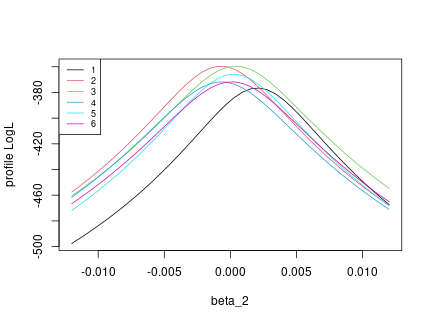
\includegraphics[width=\maxwidth]{figure/matplot_beta-1} 

}

\caption[profile log-Likelihoods of slope parameter for six covariance parameter sets]{profile log-Likelihoods of slope parameter for six covariance parameter sets}\label{fig:matplot_beta}
\end{figure}

\end{knitrout}
% swissrain matplot over betas

%meuse data
\begin{knitrout}
\definecolor{shadecolor}{rgb}{1, 1, 1}\color{fgcolor}\begin{kframe}
\begin{verbatim}
## [1] "data.frame"
## [1] "SpatialPointsDataFrame"
## attr(,"package")
## [1] "sp"
##                    estimate   ci0.005 ci0.995
## (Intercept)         0.91634  0.121205   1.711
## sqrtdist           -0.08445 -1.623508   1.455
## sdNugget            0.00785  0.000379   0.163
## sdSpatial           0.01250  0.000690   0.227
## range             173.16439 92.775636 323.209
## shape               4.00000 -9.880685  17.881
## anisoRatio          2.30106  1.138810   4.649
## anisoAngleRadians   0.27490 -0.167582   0.717
## anisoAngleDegrees  15.75042 -9.601751  41.103
## boxcox             -0.90390 -2.558961   0.751
##            nugget          variance             range 
##             0.395             1.000           173.164 
##             shape        anisoRatio anisoAngleRadians 
##             4.000             2.301             0.275 
##            boxcox 
##            -0.904
\end{verbatim}
\end{kframe}
\end{knitrout}

\pkg{gpuBatchMatrix} give wider ci and more accurate MLE's, expecially for the shape parameter.







%meuse data










\section{A simulation study}



\section{Discussion}










\bibliographystyle{unsrt}  
\bibliography{paper2}  



\end{document}


